\documentclass[tikz,border=10pt]{standalone}
\usepackage{amsmath}
\usepackage{tikz}
\usetikzlibrary{arrows.meta, positioning, calc, shapes.geometric}

\begin{document}
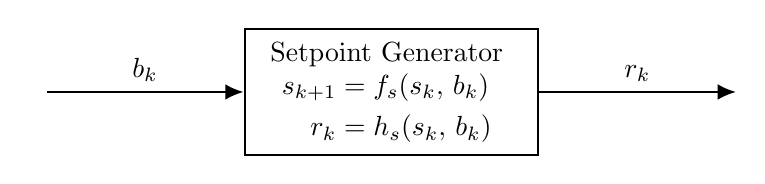
\begin{tikzpicture}[
  block/.style = {draw, thick, minimum height=3em, minimum width=6em, align=center},
  arrow/.style = {thick, -{Latex[width=2mm]}},
  node distance=2.5cm and 2.5cm
]

  % Signal Generator
  \node[block] (siggen) {
    \begin{tabular}{c}
            Setpoint Generator \\
      $\begin{aligned}
      s_{k+1} &= f_s(s_k,\,b_k) \\
      r_k &= h_s(s_k,\,b_k)
       \end{aligned}$
    \end{tabular}
  };


      % bk -> signal
  \node[left=2.5cm of siggen] (button) {};
  \draw[arrow] (button.east) -- node[above] {$b_k$} (siggen.west);
  
  \draw[arrow] (siggen.east) -- ++(2.5,0) node[midway,above] {$r_k$};




\end{tikzpicture}
\end{document}  
